\documentclass[nofootinbib,reprint,english]{revtex4-1}

% language
\usepackage[utf8]{inputenc}
\usepackage[english]{babel}

% standard setup
\usepackage{physics,amssymb,array}
\usepackage{xcolor,graphicx,hyperref}
\usepackage{tikz,listings,multirow}
\usepackage{algpseudocode,algorithm}
\usepackage{subcaption}
\usepackage{enumitem}

% tikz libraries
\usetikzlibrary{matrix}

% hyperref coloring
\hypersetup{ %
  colorlinks,
  linkcolor={red!50!black},
  citecolor={blue!50!black},
  urlcolor={blue!80!black}}

% lstlisting coloring
\lstset{ %
  inputpath=,
  backgroundcolor=\color{white!88!black},
  basicstyle={\ttfamily\scriptsize},
  commentstyle=\color{magenta},
  language=Python,
  tabsize=2,
  numbers=left,
  stringstyle=\color{green!55!black},
  frame=single,
  keywordstyle=\color{blue},
  showstringspaces=false,
  columns=fullflexible,
  keepspaces=true}

\DeclareTextSymbolDefault{\dh}{T1}

% no "do"'s or "then"'s
\algdef{SE}[FOR]{NoDoFor}{EndFor}[1]{\algorithmicfor\ #1}{\algorithmicend\ \algorithmicfor}
\algdef{SE}[FORALL]{NoDoForAll}{EndFor}[1]{\algorithmicfor\ #1}{\algorithmicend\ \algorithmicfor}
\algdef{SE}[IF]{NoThenIf}{EndIf}[1]{\algorithmicif\ #1}{\algorithmicend\ \algorithmicif}

% spin-configuration table columns
\newcolumntype{M}[1]{>{\centering\arraybackslash}m{#1}}
\newcolumntype{N}{@{}m{0pt}@{}}

% shortcuts


\begin{document}
% titlepage
\title{FYS3150 Machine Learning - Project 3\\Classifying Pulsar Candidates With Machine Learning Methods}
\author{Nils Johannes Mikkelsen}
\date{\today}
\noaffiliation
\begin{abstract}

\end{abstract}
\maketitle
All material for project 3 may be found at:\\
{\scriptsize\url{https://github.com/njmikkelsen/machinelearning2018/tree/master/Project3}}
\section{Introduction}

\section{Theory}
\subsection{Radio Analysis of Pulsars}
The following theory is mostly based on F.G. Smith's 1977 \emph{Pulsars} \cite{Pulsars}, with additional information taken from ``Chapter 6: Pulsars'' of Jim Condon's online book \emph{Essential Radio Astronomy} \cite{EssentialRadioAstronomy}.
\subsubsection{The basics of pulsars}
Pulsars are heavily magnetised rotating astronomical objects that emit regular pulses of electromagnetic (EM) radiation. Initially discovered in 1967 by Antony Hewish and Jocelyn Bell Burnell, it is generally believed by most modern astronomers that pulsars are neutron stars, the product of some supernovae. There are several mechanims that result in the electromagnetic radiation (although still not entirely understood), astronomers have thus devised three major categories of pulsars according to the source of radiation: rotation-powered pulsars, accretion-powered pulsars and magnetars. Rotation-powered pulsars use the loss of rotational energy, accretion-powered pulsars exploit the gravitational potential energy of accreted matter, while magnetars are believed to power its radiation pulses by the decay of an extremely strong magnetic field (\(\sim10^{10}\) T). Other than regular pulses of radiation, the properties of the radiation from the different categories are mostly different. Rotation-powered pulsars radiate mostly in the Radio spectrum, while the accretion-powered pulsars radiate mostly in the X-Ray spectrum. Magnetars have been observed to radiate both in the X-Ray and gamma-ray spectra.

The data studied in this project stem from radio-telescope observations, thus only rotation-powered pulsars are considered here.
\subsubsection{ISM dispersion}
As the name implies, radio pulsars are particular pulsars that radiate in the radio spectrum. When astronomers first began studying radio pulsars they noticed that radiation from the same pulsar with different frequencies arrived on Earth at different times. It was quickly pointed out that this EM dispersion coincided with the expected dispersion of EM waves travelling through the cold plasma of the interstellar medium (ISM). Travelling through an ionised gas, the group and phase velocities of radio waves, \(v_g\) and \(v_p\) respectively, are related by
\begin{equation}\label{eq:group_and_phase_velocities_cold_plasma}
v_gv_p=c^2
\end{equation}
where \(c\) is the speed of light in a vacuum. The fractive index of the cold plasma is
\begin{equation}\label{eq:refractive_index_cold_plasma}
\mu=\sqrt{1-\Big(\frac{\nu_\text{p}}{\nu}\Big)^2}
\end{equation}
where \(\nu\) is the radio wave frequency and \(\nu_\text{p}\) is the \emph{plasma frequency} given by:
\begin{equation}
\nu_\text{p}=\sqrt{\frac{e^2n_e}{\pi m_e}}
\end{equation}
Here, \(n_e\) and \(m_e\) are the electron number density and \(m_e\) is the electron mass. Now, radio waves with \(\nu\leq\nu_\text{p}\) are unable to propegate through the ISM. On the other hand, waves with \(\nu>\nu_\text{p}\) do propegate through the ISM with a group velocity of
\begin{equation}\label{eq:radio_wave_group_velocity_propegation}
v_g=\mu c\cong\bigg(1-\frac{\nu_\text{p}^2}{2\nu^2}\,\bigg)c
\end{equation}
Hence, the travel time \(T\) spent by a radio pulse from a pulsar a distance \(L\) away is
\begin{align}
T&=\int_0^L\frac{1}{v_g}\dd{l}=\frac{1}{c}\int_0^L\bigg(1+\frac{\nu_\text{p}^2}{2\nu}\bigg)\dd{l}\nonumber\\
&=\frac{d}{c}+\bigg(\frac{e^2}{2\pi m_ec}\bigg)\nu^{-2}\int_0^L n_e\dd{l}\label{eq:radio_wave_travel_time}
\end{align}
The integral in \eqref{eq:radio_wave_travel_time} is commonly called the \emph{Dispersion Measure}, and is commonly given in units of pc \(\text{cm}^{-3}\):
\begin{equation}\label{eq:Dispersion_Measure}
\text{DM}=\int_0^Ln_e\dd{l}
\end{equation}
The Dispersion Measure is not a trivial quantity to estimate because it depends on the constituents and their arrangements of the ISM, which in general is not uniform. Despite accurate theoretical predictions of DM, it continues to be an essential variable parameter in radio astronomy analysis, more or this below. In astronomy-convenient units, the dispersion delay \(t=T-d/c\) due to the ISM is
\begin{equation}\label{eq:ISM_dispersion_delay}
t\cong4.149\cdot10^3\nu^{-2}\,\text{DM}\text{ seconds}
\end{equation}
where \(\nu\) in MHz and DM in pc \(\text{cm}^{-3}\).
\subsubsection{The integrated pulse profile}
Due to difficulties with time-resolution, limited bandwidth, etc., studying a single radio pulse is considerably more difficult than to study the ``average pulse'' across several frequencies. Taking into account the time delay due to dispersion in the ISM (equation \eqref{eq:ISM_dispersion_delay}), the radio pulses from radio pulsars may be \emph{folded} to yield an integrated pulse profile. Seeing that the DM is essential in the computation of the time delay, astronomers often study the integrated pulse profile as a function of DM. An example of the folding process is shown in figure \ref{fig:integrated_pulse_profile}, note that the delay folds across several pulse periods. Moreover, while the time-signal is fairly chaotic, the integrated pulse profile is very focused.

While all pulsars share the property of a stable pulse profile, it turns out that each pulsar exhibits a particular profile that is more or less unique. This unique profile, often nicknamed the ``fingerprint'' of the pulsar, can have several peaks and be less or more spread out. Nonetheless, some statistical properties such as a single peak, a double peak, various minor peaks, etc., do occur quite frequently.

\begin{figure}
\centering
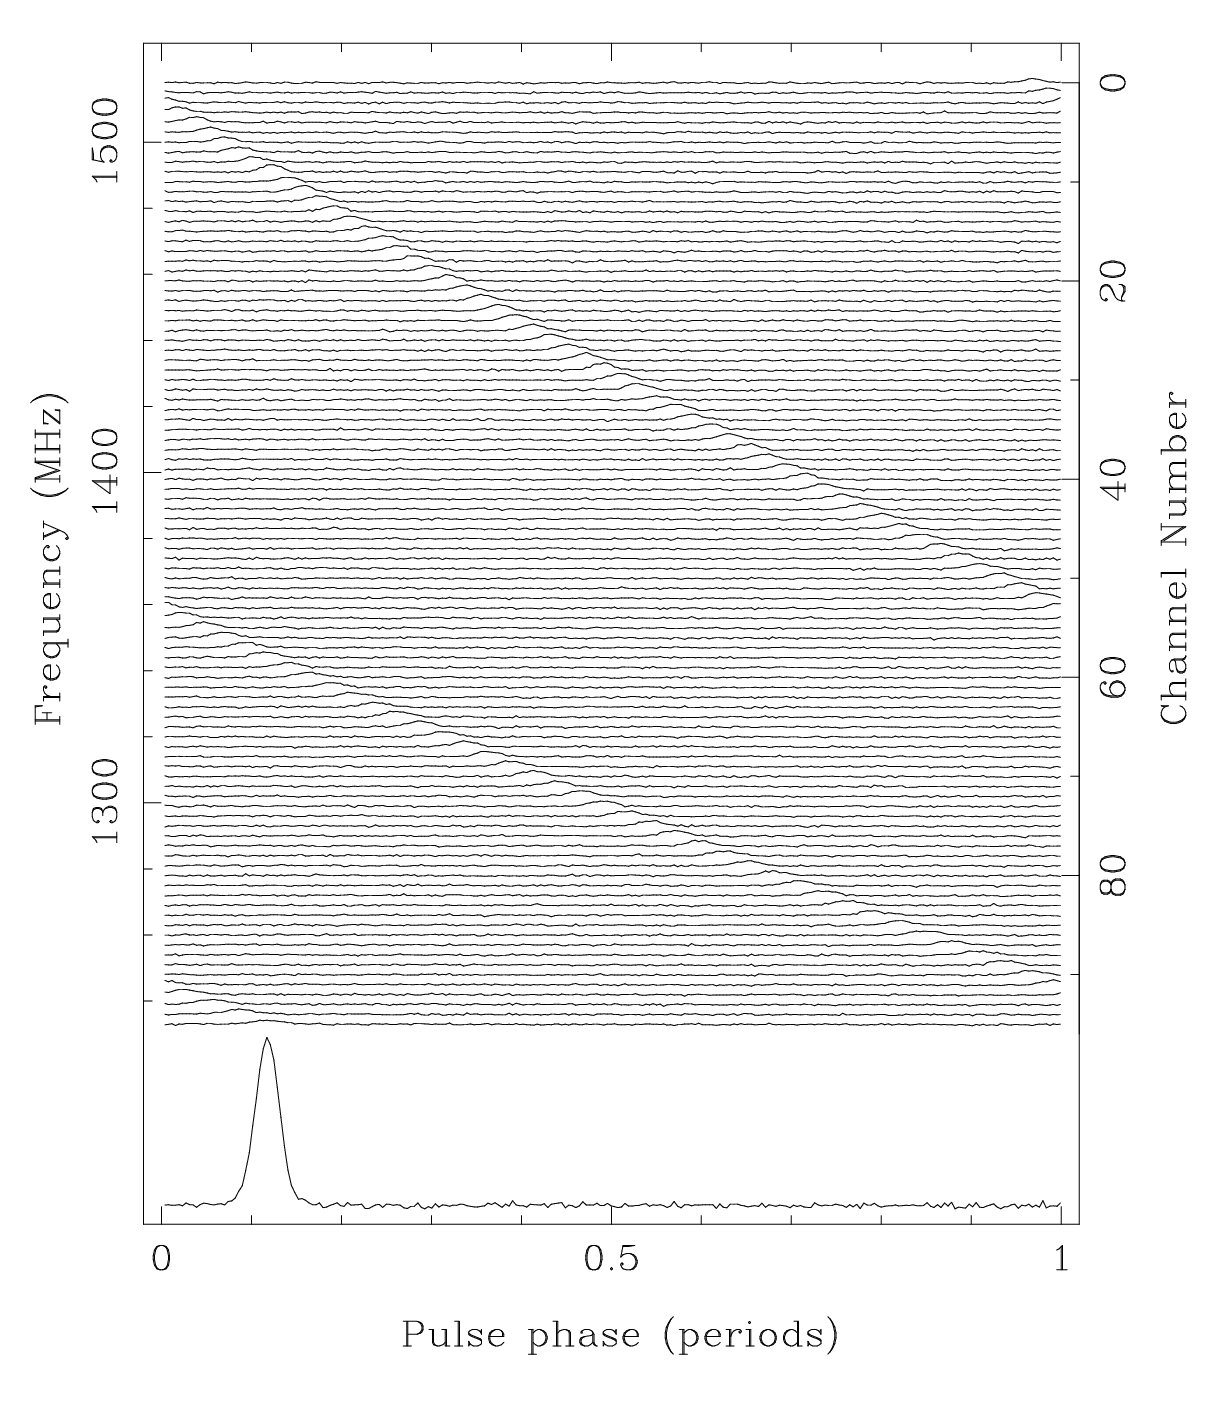
\includegraphics[scale=0.2]{./Pulsar_dm.png}
\caption{The pulse profile of a radio wave experiences a time delay due to dispersion in the ISM. The integrated pulse profile is a folded profile that finds an average pulse profile by taking into account the time delay. Source: \cite{IntegratedPulseProfile}}\label{fig:integrated_pulse_profile}
\end{figure}

\subsubsection{Signal-to-noise ratio}
An important quantity in observational astronomy is the Signal-to-Noise Ratio (SNR), which in its simplest form is defined as the ratio of the power of the signal to the power of the noise:
\begin{equation}
\text{SNR}=\frac{P_\text{signal}}{P_\text{noise}}
\end{equation}
SNR is a measure of the quality of observation, or ``amount of meaningful information'' in an observation. Astronomers actually use the SNR to study the DM parameter space, as selecting the optimal DM is essential for conducting a proper analysis of the integrated pulse profile. Enter the the DM-SNR curve: the SNR score of an integrated pulse profile as a function of DM. The DM-SNR curve is usually flat for non-pulsating signals, however peaks about the optimal DM if the signal does pulsate. Consequently, the DM-SNR curve is commonly used as a preliminary test for identifying signals from pulsars in large data sets of radio signals.

\subsection{Moments In Statistics}
Given some continuous function \(f:\mathbb{R}\to\mathbb{R}\), its \(n^\text{th}\) \emph{moment} \(\mu_n(c)\) about the real value \(c\) is defined as
\begin{equation}\label{eq:moments}
\mu_n(c)=\int_{-\infty}^\infty(x-c)^nf(x)\dd{x}
\end{equation}
Moments are used in several areas of science and mathematics, most prominently in mechanics and probability theory. If \(f\) is a probability density (or strictly non-negative and normalizable),\footnote{A probability density \(f:D\to\mathbb{R}\) satifies
\[0\leq f(x),\ \forall x\in D\qand\int_Df(x)\dd{x}=1.\]
Note that \(D\) is usually the entire real number line.} there exists two major notation conventions:
\[\mu_n(c)=E\big[(X-c)^n\big]\qand\mu_n(c)=\expval{(x-c)^n}\]
The former is favoured by statisticians, while the latter is favoured by physicists, this project will employ the physicists' convention.

The moments most often studied in probability theory are the so-called \emph{central} moments \(\mu_n\):
\begin{equation}\label{eq:central_moments}
\mu_n=\mu_n(\mu)=\expval{(x-\mu)^n}=\int_{-\infty}^\infty(x-\mu)^nf(x)\dd{x}
\end{equation}
where \(\mu=\expval{x}\) is the mean value of the distribution and \(\mu_n=\mu_n(\mu)\) is introduced to simplify notation. The \(0^\text{th}\) and \(1^\text{st}\) central moments are 1 and 0 respectively as \(f(x)\) is normalized and \((x-\mu)f(x)\) is centered about \(\mu\). The \(2^\text{nd}\) central moment is the variance:
\begin{equation}
\mu_2=\expval{(x-\mu)^2}=\sigma^2
\end{equation}
where \(\sigma\) is the standard deviation.

Furthermore, the central moments are used to define the \emph{normalized} moments \(\tilde{\mu}_n\):
\begin{equation}
\tilde{\mu}_n=\frac{\mu_n}{\sigma^n}=\frac{\expval{(x-\mu)^n}}{\expval{(x-\mu)^2}^{n/2}}
\end{equation}
Normalized moments are dimensionless quantities that describe the underlying distribution independently of the scale of the data. The \(3^\text{rd}\) normalized moment is known as the \emph{skewness} of a distribution and quantifies the extent to which a distribution is \emph{skewed} to ``left or right'' of the mean. Positive skewness implies the distribution is skewed towards \(x\) values greater than \(\mu\) and vice versa. The \(4^\text{th}\) normalized moment is called \emph{kurtosis} and is a measure of how quickly the tails of a distribution tends to zero, i.e. a measure of ``\emph{peakness}''. Kurtosis is usually reported as \emph{excess kurtosis}, which is the kurtosis of a distribution relative to the normal distribution (whose kurotsis is 3). Hence the definition:
\begin{equation}
\text{Excess Kurtosis }=\text{ Kurtosis}-3
\end{equation}
\subsection{Machine Learning - Artificial Neural Networks}
Artificial Nerual Networks (ANN or simply NN) is a Supervised Machine Learning (SML) technique that is inspired by biological neural networks in animal brains. Rather than a specific technique or algorithm, ANN is an umbrella term for several NN structures and algorithms whose complexity, computational difficulty, etc., varies greatly between different techniques.
\subsubsection{The Multi-Layered Perceptron}
This project will employ the so-called Multi-Layered Perceptron (MLP) model, which is a particular ANN that is based around the idea of organizing the network's neurons, or nodes, in layers. A node is loosely based on the concept of biological neuron, which is capable of recieving an electrical signal, process it, and transmit a new signal to other neurons. In the MLP model the neurons are arranged in \(L\) consecutive layers with \(N_l\) number of nodes per layer (unqeual number of nodes per layer is alloweed).  There are three types of layers: input, hidden and output layers. The input and output layers manage the network's inputs and outputs, while the hidden layers serve as the network's data-processing backbone. Particular to the MLP, every node in each hidden layer is connected to every node in the previous and the next layers, but nodes within the same layer are \emph{not} connected. The MLP structure is illustrated in figure \ref{fig:node_connections}, note the inclusion of ``bias'': Bias is an additional property of all layers except the input layer whose purpose is essentially to center the data about 0. Conceptually, one may think of bias as the role of the intercept in Linear Regression analysis.

\begin{figure}
\centering
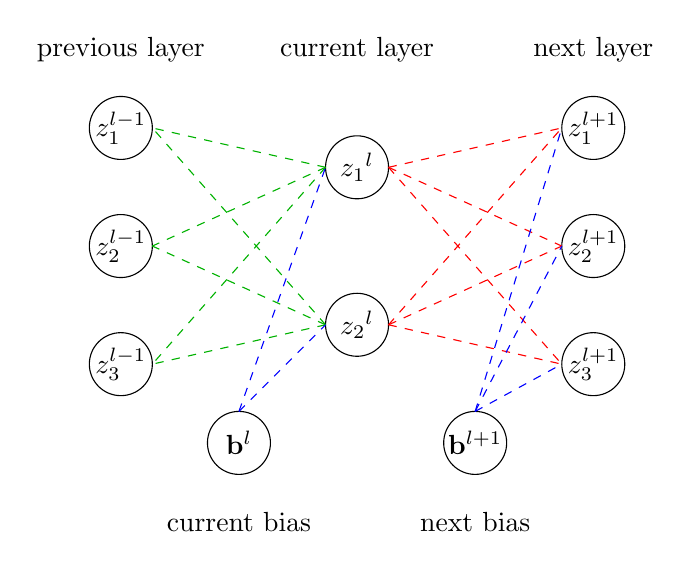
\begin{tikzpicture}
% NODES
\draw node at (-3,2.5) {previous layer};
\draw (-3,+1.5) circle [radius=0.4];
\draw (-3,+0.0) circle [radius=0.4];
\draw (-3,-1.5) circle [radius=0.4];

\draw node at (-1.5,-3.5) {current bias};
\draw (-1.5,-2.5) circle [radius=0.4];

\draw node at (+0,2.5) {current layer};
\draw (+0,+1.0) circle [radius=0.4];
\draw (+0,-1.0) circle [radius=0.4];

\draw node at (+1.5,-3.5) {next bias};
\draw (+1.5,-2.5) circle [radius=0.4];

\draw node at (+3,2.5) {next layer};
\draw (+3,+1.5) circle [radius=0.4];
\draw (+3,+0.0) circle [radius=0.4];
\draw (+3,-1.5) circle [radius=0.4];
% CONNECTIONS
\draw[dashed,red] (+0.4,+1.0) -- (+3-0.4,+1.5);
\draw[dashed,red] (+0.4,+1.0) -- (+3-0.4,+0.0);
\draw[dashed,red] (+0.4,+1.0) -- (+3-0.4,-1.5);

\draw[dashed,red] (+0.4,-1.0) -- (+3-0.4,+1.5);
\draw[dashed,red] (+0.4,-1.0) -- (+3-0.4,+0.0);
\draw[dashed,red] (+0.4,-1.0) -- (+3-0.4,-1.5);

\draw[dashed,green!70!black] (-0.4,+1.0) -- (-3+0.4,+1.5);
\draw[dashed,green!70!black] (-0.4,+1.0) -- (-3+0.4,+0.0);
\draw[dashed,green!70!black] (-0.4,+1.0) -- (-3+0.4,-1.5);

\draw[dashed,green!70!black] (-0.4,-1.0) -- (-3+0.4,+1.5);
\draw[dashed,green!70!black] (-0.4,-1.0) -- (-3+0.4,+0.0);
\draw[dashed,green!70!black] (-0.4,-1.0) -- (-3+0.4,-1.5);

\draw[dashed,blue] (+1.5,-2.5+0.4) -- (+3.0-0.4,+1.5);
\draw[dashed,blue] (+1.5,-2.5+0.4) -- (+3.0-0.4,+0.0);
\draw[dashed,blue] (+1.5,-2.5+0.4) -- (+3.0-0.4,-1.5);

\draw[dashed,blue] (-1.5,-2.5+0.4) -- (-0.4,+1.0);
\draw[dashed,blue] (-1.5,-2.5+0.4) -- (-0.4,-1.0);
% NODE NAMES
\draw node at (+0.0,+1.0) {\({z_1}^l\)};
\draw node at (+0.0,-1.0) {\({z_2}^l\)};

\draw node at (+3.0,+1.5) {\(z_1^{l+1}\)};
\draw node at (+3.0,+0.0) {\(z_2^{l+1}\)};
\draw node at (+3.0,-1.5) {\(z_3^{l+1}\)};

\draw node at (-3.0,+1.5) {\(z_1^{l-1}\)};
\draw node at (-3.0,+0.0) {\(z_2^{l-1}\)};
\draw node at (-3.0,-1.5) {\(z_3^{l-1}\)};

\draw node at (+1.5,-2.5) {\(\vb{b}^{l+1}\)};
\draw node at (-1.5,-2.5) {\(\vb{b}^l\)};
\end{tikzpicture}
\caption{An illustration of the structure of an MLP ANN: Each node is connected to every node in the previous layer and the next layer. The inputs to the current layer consists of the data from the previous layer (green connections) and the current layer's bias (left blue connections). The outputs of the current layer (red connections) together with the next layer's bias (right blue connections) become the inputs of the next layer, and so on.}\label{fig:node_connections}
\end{figure}

So far the network has only been described using fluid terms such as ``transfer of information'' and ``node connections'', this will be expanded upon now. The number of nodes in the input layer \(N_1\) must exactly match the dimensionality of the input data, thus there is a one-to-one correspondence between the nodes and the indices of the input data (usually a vector quantity). Similarly, the number of nodes in output layer \(N_L\) must exactly match the output data of the network, again with a one-to-one correspondence between nodes and data indices. It follows that in practice it is really only the hidden layers that may have a variable number of nodes \(N_l\), \(l\in\{2,\ldots,L-1\}\). The network processes input data layer-by-layer, meaning each hidden layer processes the data in sequence. Data from the input layer is sent to the first hidden layer, processed, then transfered to the next layer, and so on.

Mathematically speaking, the connection between two nodes \(i\) in layer \(l\) and \(j\) in layer \(l+1\) is a scaling operation. The connection's scaling factor is usually called the weight and is commonly denoted by \(w_{ij}^{l+1}\), note the convention of labeling a connection weight between layers \(l\) and \(l+1\) by \(l+1\). Each node is connected to every node in the previous layer, thus the purpose of weighting the data is to regulate the importance of each node in the previous layer. However, note that unless some other operation is conducted on the data the network's overall operation on the input data is only linear (meaning methods such as Linear Regression are more appropriate). This is circumvented by the addition of a non-linear operation on the every node's input, commonly called the node's \emph{activation} function. Common choices of activations are the sigmoid function and the tangent hyperbolicus:
\begin{subequations}
\begin{align}
\text{sigmoid}(x)&=\frac{1}{1+e^{-x}}\\
\tanh(x)&=\frac{e^x-e^{-x}}{e^x+e^{-x}}
\end{align}
\end{subequations}
Other activation functions are also used. Technically, a network may have a different activation for each node, but this is rarely done in practice. On the other hand, layer-wide activation functions are often implemented, so much so that the following theory will base the mathematics on the presumption of layer-wide activation.

The data in node \(i\) in layer \(l\) is denoted by \(y_i^l\). The connection weight between node \(i\) in layer \(l\) and node \(j\) in layer \(l+1\) is denoted by \(w_{ij}^{l+1}\). The accumulated data input from all nodes in layer \(l\) received by node \(j\) in layer \(l+1\), adjusted for bias \(b_j\), is given by
\begin{equation}\label{eq:neural_network_node_received_data}
z_j^{l+1}=\sum_{i=1}^{N_l}w_{ij}^{l+1}y_i^l+b_i^l
\end{equation}
The input data received by the node is \(f_{l+1}(z_j^{l+1})\), where \(f_{l+1}\) is the activation function of layer \(l+1\). Hence, the data in node \(j\) in layer \(l+1\) is given by
\begin{equation}\label{eq:neural_network_node_data}
y_j^{l+1}=f_{l+1}(z_j^{l+1})=f_{l+1}\Bigg(\sum_{i=1}^{N_l}w_{ij}^{l+1}y_i^l+b_j^{l+1}\Bigg)
\end{equation}
Arranging the node data in vectors \(\vb{y}^l\), the node inputs in vectors \(\vb{z}^{l+1}\), the connection weights in a weight matrix \(\hat{W}^{l+1}\) and the bias in bias vectors \(\vb{b}^{l+1}\), then \eqref{eq:neural_network_node_data} can be reformulated as a layer-wide (matrix) operation:
\begin{equation}\label{eq:neural_network_layer_input}
\vb{y}^{l+1}=f_{l+1}(\vb{z}^{l+1})=f_{l+1}\Big(\hat{W}^{l+1}\vb{z}^l+\vb{b}^{l+1}\Big)
\end{equation}
To conclude this section: The answer to the question \emph{"What is a Multi-Layered Perceptron Neural Network?"} is the following function:
\begin{equation}\label{eq:equation_of_neural_network}
\vb{y}=f_L\bigg(\hat{W}^Lf_{L-1}\bigg(\cdots \bigg(\hat{W}^1\vb{x}+\vb{b}^1\bigg)\cdots\bigg)+\vb{b}^L\bigg)
\end{equation}
where \(\vb{x}=\vb{y}^1\) and \(\vb{y}=\vb{y}^L\) are the network's inputs and outputs.
\subsubsection{Training an MLP}
The basis of the MLP, and many similar network structures, is the so-called \emph{back-propagation} algorithm (BPA). The MLP is an example of a \emph{supervised} machine learning technique, meaning the desired outputs are known. In case of the MLP, it is the BPA that introduces supervision.

At its core, the BPA is essentially a variant of gradient descent techniques. The basic problem of gradient descent methods is to find the input \(\vb{x}_\text{min}\in D\) that minimises some function \(F:D\to\mathbb{R}\). The algorithm is based on producing sucessive approximations of \(\vb{x}_\text{min}\), each closer to the true minium. Seeing that the goal is to minimise \(F\), the direction of each step is chosen opposite of the gradient of \(F\). The fundamental algorithm is summarised below:
\begin{algorithm}[H]
\caption{Gradient Descent}\label{alg:gradient_descent}
\begin{algorithmic}[1]
\State Select a trial input \(\vb{x}_0\).
\NoDoFor {\(i=1,\ldots,N\):}
	\State Compute: \(\displaystyle\vb{x}_i=\vb{x}_{i-1}-\gamma_n\pdv{F}{\vb{x}}\eval_{\vb{x}_{i-1}}\)
\EndFor
\end{algorithmic}
\end{algorithm}
\noindent Note that the derivative is not scalar. The step length \(\gamma_n\) may be variable or constant depending on the implementation, although proper convergence is impossible with too large steps.

The \(F\) function to minimise in the BPA is the so-called \emph{cost} function, denoted \(C\). Similar to activation functions, different cost functions are used in different problems. The cost function most used in classification analysis is the so-called cross-entropy:
\begin{equation}\label{eq:cross_entropy_MLP}
C(\vb{y}|\vb{t})=-\Big[\vb{t}^T\ln(\vb{y})+(1-\vb{t})^T\ln(1-\vb{y})\Big]
\end{equation}
where \(\vb{y}\) is a vector of the network's outputs and \(\vb{t}\) is a vector of the targets, i.e. the desired network output.\footnote{The introduction of \(\vb{t}\) in the cost function is the actual introduction of machine learning supervision in MLP ANNs. Also, note that naming \(\vb{t}\) the ``targets'' refers to the goal of neural networks: namely to construct the network such that it reproduces the target outputs.} Note that \(C(\vb{y}|\vb{t})\) is univariate: it is a function of outputs \(\vb{y}\) provided the targets \(\vb{t}\) (that is, \(\vb{t}\) is not a variable quantity). The derivative of \(C(\vb{y}|\vb{t})\) is
\begin{equation}\label{eq:cross_entropy_derivative_MLP}
\pdv{C}{\vb{y}}=(\vb{y}-\vb{t})\oslash\Big(\vb{y}\circ(1-\vb{y})\Big)
\end{equation}
where \(\oslash\) and \(\circ\) denotes the Hadamard division and product (element-wise operations). Now, if this was a problem for gradient descent methods, then \(\vb{y}\) would be updated directly using Algorithm \ref{alg:gradient_descent} and equation \eqref{eq:cross_entropy_derivative_MLP}. However, \(\vb{y}\) is produced by the network according to equation \eqref{eq:equation_of_neural_network}, which is dependent on the weights and biases of each layer. Hence, in order for the BPA to improve the network it must study \(C(\vb{y}|\vb{t})\) with respect to all weights and biases. 

Although seemingly difficult, the problem is actually somewhat straight-forward, it all comes down to clever use of the chain rule and limiting the number of necessary computations. Observe that the derivative of \(C(\vb{y}|\vb{t})\) with respect to layer \(l\) can be written as
\begin{subequations}\label{eq:cost_derivative_layer_l_standard}
\begin{align}
\pdv{C}{\hat{W}^l}&=\pdv{C}{\vb{y}^l}\,\pdv{\vb{y}^l}{\vb{z}^l}\,\pdv{\vb{z}^l}{\hat{W}^l}\\
\pdv{C}{\vb{b}^l}&=\pdv{C}{\vb{y}^l}\,\pdv{\vb{y}^l}{\vb{z}^l}\,\pdv{\vb{z}^l}{\vb{b}^l}
\end{align}
\end{subequations}
Now define the \emph{signal error} of layer \(l\) as
\begin{equation}\label{eq:signal_error_definition}
\hat{\delta}^l\equiv\pdv{C}{\vb{z}^l}=\pdv{C}{\vb{y}^l}\,\pdv{\vb{y}^l}{\vb{z}^l}=\pdv{C}{\vb{y}^l}\circ f'_l(\vb{z}^l)
\end{equation}
where \(f'_l(\vb{z}^l)\) is the derivative of the activation function of layer \(l\). Clearly then equations \eqref{eq:cost_derivative_layer_l_standard} may be written as
\begin{subequations}\label{eq:cost_derivative_layer_l}
\begin{align}
\pdv{C}{\hat{W}^l}&=\hat{\delta}^l\vb{y}^{l-1}\\
\pdv{C}{\vb{b}^l}&=\hat{\delta}^l
\end{align}
\end{subequations}
where \(\vb{z}^l=\hat{W}^l\vb{y}^{l-1}+\vb{b}^l\) was used to evalute \(\partial\vb{z}^l/\partial\hat{W}^l\) and \(\partial\vb{z}^l/\partial\vb{b}^l\). The next step is to relate the signal error of layer \(l\) to \(l+1\), the idea to rewrite \(\partial C/\partial\vb{y}^l\) in \eqref{eq:signal_error_definition} using a reverse chain rule:\footnote{The awkward double-transpose notation is used to preserve the correct dimensions of \(\partial C/\partial\vb{y}^l\).}
\[\pdv{C}{\vb{y}^l}=\pdv{C}{\vb{z}^{l+1}}\,\pdv{\vb{z}^{l+1}}{\vb{y}^l}=\Big[\big(\hat{\delta}^{l+1}\big)^T\hat{W}^{l+1}\Big]^T=\big(\hat{W}^{l+1}\big)^T\hat{\delta}^{l+1}\]
That is, the signal error of layer \(l\) is related to the signal error of layer \(l+1\) via
\begin{equation}\label{eq:signal_error_recursive_relation}
\hat{\delta}^l=\big(\hat{W}^{l+1}\big)^T\hat{\delta}^{l+1}\circ f'_l(\vb{z}^l)
\end{equation}

Equations \eqref{eq:cost_derivative_layer_l}, \eqref{eq:signal_error_definition} and \eqref{eq:signal_error_recursive_relation} are what constitutes the \emph{four equations of the back-propagation algorithm}. The equations essentially boil down to the equivalent of step 3 in Algorithm \ref{alg:gradient_descent} (in particular \eqref{eq:cost_derivative_layer_l}). Moreover, note that the ``back-propagated quantity'' in the BPA is the signal error, i.e., the network's output error is propegated backwards through the network (thereby expressing the dependency of the cost function on the signal error of the different layers).

The back-propagation algorithm is composed of 3 steps: the feed forward cycle, the back-propagation and the network update. The feed forward step refers to the computation of the network's output; the input data \(\vb{x}\) is ``fed forward'' to the output. The back-propagation step involves the computation of the signal errors and the final network update is the updating of the network's weights and biases using the derivatives of the cost function. The full algorithm is shown below. 

\begin{algorithm}[H]
\caption{The Back-Propagation Algorithm}\label{alg:back_propagation}
\begin{algorithmic}[1]
\State Initiate the network weights and biases.
\NoDoFor {\(i=1,\ldots,N\):}
	\State Feed forward input \(\vb{x}\).
	\State Compute \(\hat{\delta}^L\).
	\NoDoFor {\(l=L-1,\ldots,1\):}
		\State Compute \(\hat{\delta}^l\).
	\EndFor
	\State Update the network weights and biases according to
\begin{align*}
\hat{W}^l_\text{next}&=\hat{W}^l_\text{prev}-\gamma_i\pdv{C}{\hat{W}^l_\text{prev}}\\
\vb{b}^l_\text{next}&=\vb{b}^l_\text{prev}-\gamma_i\pdv{C}{\vb{b}^l_\text{prev}}
\end{align*}
\EndFor
\end{algorithmic}
\end{algorithm}

\subsection{Machine Learning - Support Vector Machines}
One of the most versatile and diverse approaches to SML is Support Vector Machines (SVM). SVMs are very popular for both regression and classification problems, this project however will only perform a binary classification. The mathematics are therefore presented with a binary labelling in mind.\footnote{SVM classification with several classes is actually just a recursive use of binary classifications. E.g. Dividing the real number line into three classes \((-\infty,0)\), \([0,10]\) and \((10,\infty)\) is the same as first dividing the real number line into \((-\infty,0)\) and \([0,\infty)\), then subdividing \([0,\infty)\) into \([0,10]\) and \((10,\infty)\).}
\subsubsection{The basic principles behind SVMs}
The basic idea of an SVM classifiers is to divide a data set into discrete classes using a \emph{decision boundary}, whose mathematical description is that of a \emph{hyperplane}. Technically speaking, hyperplanes are affine subspaces that represent the direct generalisation of the concept of two-dimensional planes located in three-dimensional spaces. It happens that any decision boundary of a \(p\)-dimensional predictor space must be a \((p-1)\)-dimensional hyperplane.

Hyperplanes may be parametrised via a linear equation using an intercept \(\beta_0\) and a parameter vector \(\hat{\beta}^T=\mqty(\beta_1&\cdots&\beta_p)\). Written in set notation, the definition of a hyperplane in a real \(p\)-dimensional space is
\begin{equation}\label{eq:hyperplane}
\text{hyperplane}=\{\vb{x}\ |\ \vb{x}^T\hat{\beta}+\beta_0=0\}
\end{equation}
This definition of a hyperplane is particularly useful, because it accounts for the two regions separated by the hyperplane by changing the equality in \(\vb{x}^T\hat{\beta}+\beta_0\) to either \(<\) or \(>\). Hence, a natural binary classification based on \eqref{eq:hyperplane} is to simply use the sign:\footnote{This classification rule actually does not include points on the decision boundary, thus common practice is to let these points belong to the positive sign class by default.}
\begin{equation}\label{eq:SVM_classification_rule}
\text{class label}=\text{sign}(\vb{x}^T\hat{\beta}+\beta_0)
\end{equation}
where the binary label (i.e. \(\pm1\)) is an arbitrary choice that simplifies notation. Note that the description of decision boundaries as hyperplanes necessarily restricts the possible boundaries to linear boundaries. It turns out that this problem is easily circumvented by introducing a benefitial transformation of the predictor space. This is done in later sections.

Suppose a particular linear decision boundary is parametrised by \(\beta_0\) and \(\hat{\beta}\). By definition, any point \(\vb{x}_i\) on the hyperplane  satisfies \(\hat{\beta}^T\vb{x}_i=-\beta_0\), and consequently any two points on the hyperplane \(\vb{x}_1\) and \(\vb{x}_2\) must therefore satisfy \(\hat{\beta}^T(\vb{x}_2-\vb{x}_1)=0\). It follows that \(\hat{\beta}/||\hat{\beta}||\) is a unit vector normal to the surface of the hyperplane. Now consider any point in the predictor space \(\vb{x}\): because the hyperplane is infinite in reach, there must exist some point on the hyperplane \(\vb{x}_0\) such that the distance from \(\vb{x}\) to \(\vb{x}_0\) is minimal. Because \(\hat{\beta}/||\hat{\beta}||\) is necessarily the unit vector pointing along the line defined by \(\vb{x}\) and \(\vb{x}_0\),\footnote{This follows from the fact that the dimensionality of the hyperplane is one less than the dimensionality of the predictor space. That is, the only degree of freedom that separates \(\vb{x}\) from \(\vb{x}_0\) is the direction of the unit vector normal to the hyperplane surface, which is \(\hat{\beta}/||\hat{\beta}||\).} the signed distance from \(\vb{x}_0\) to \(\vb{x}\) must satisfy
\begin{equation}
\frac{\hat{\beta}^T}{||\hat{\beta}||}(\vb{x}-\vb{x}_0)=\frac{1}{||\hat{\beta}||}(\hat{\beta}^T\vb{x}+\beta_0)
\end{equation}
That is, the signed distance from any data point \(\vb{x}\) to \(\vb{x}_0\) on the decision boundary is proportional to \(\hat{\beta}^T\vb{x}+\beta_0\). The smallest distance between any data point and the decision boundary is called the decision boundary's \emph{margin} \(M\). The mission statement of SVMs is to find a hyperplane (i.e. determine \(\hat{\beta}\) and \(\beta_0\)) that maximises the margin. Using the class labelling
\begin{equation}
y_i=\begin{cases}+1,&\vb{x}_i^T\hat{\beta}+\beta_0\geq0\\-1,&\vb{x}_i^T\hat{\beta}+\beta_0<0\end{cases}
\end{equation}
the SVM mission statement may be expressed as an optimization problem:
\begin{equation}\label{eq:SVM_optimization_problem}
\frac{y_i}{||\hat{\beta}||}(\vb{x}_i^T\hat{\beta}+\beta_0)\geq M\qc i\in\{1,\ldots,N\}
\end{equation}
or alternatively if \(||\hat{\beta}||=1/M\):
\begin{equation}\label{eq:SVM_optimization_problem_Lagrange_form}
\min_{\hat{\beta},\beta_0}\frac{1}{2}||\hat{\beta}||\qq{subject to }y_i(\vb{x}_i^T\hat{\beta}+\beta_0)\geq1\qc\forall i
\end{equation}
This is an example of a convex optimization problem, and is appropriately studied using the method of Lagrange multipliers.

The Lagrangian primal to be minimized is
\begin{equation}\label{eq:SVM_Lagrangian_primal}
\mathcal{L}(\hat{\beta},\beta_0,\hat{\lambda})=\frac{1}{2}||\hat{\beta}||^2-\sum_{i=1}^N\lambda_i\big(y_i(\vb{x}_i^T\hat{\beta}+\beta_0)-1\big)
\end{equation}
Its derivatives are
\begin{subequations}
\begin{align}
\pdv{\mathcal{L}}{\hat{\beta}}&=\hat{\beta}-\sum_{i=1}^N\lambda_iy_i\vb{x}_i\\
\pdv{\mathcal{L}}{\beta_0}&=-\sum_{i=1}^N\lambda_iy_i
\end{align}
\end{subequations}
Setting \(\partial\mathcal{L}/\partial\hat{\beta}=0\) and \(\partial\mathcal{L}/\partial\beta_0=0\), then inserting the results back into \eqref{eq:SVM_Lagrangian_primal} one finds the Wolfe dual (a maximization problem):
\begin{subequations}\label{eq:SVM_Wolfe_dual}
\begin{align}
&\mathcal{L}(\hat{\lambda})=\sum_{i=1}^N\lambda_i-\frac{1}{2}\sum_{i=1}^N\sum_{j=1}^N\lambda_i\lambda_iy_iy_j\vb{x}_i^T\vb{x}_j\label{eq:SVM_Wolfe_dual_a}\\
&\text{subject to }\lambda_i\geq0\qand\sum_{i=1}^N\lambda_iy_i=0
\end{align}
\end{subequations}
In addition to the constraints of the Wolfe dual, the solution must also satisfy the so-called KKT (Karush-Kuhn-Tucker) conditions:
\begin{equation}\label{eq:SVM_KKT_condition}
\lambda_i\big(y_i(\vb{x}_i^T\hat{\beta}+\beta_0)-1\big)=0\qc\forall i
\end{equation}
It follows from \eqref{eq:SVM_KKT_condition} that either of two events is possible: If \(\lambda_i>0\), then it must be so that \(y_i(\vb{x}^T\hat{\beta}+\beta_0)=1\), in which case \(\vb{x}_i\) is on the boundary. Else, if \(y_i(\vb{x}^T\hat{\beta}+\beta_0)>1\), then \(\lambda_i=0\) and \(\vb{x}_i\) is not on the boundary. Due to the particular role of the \(\vb{x}_i\) vectors in the Wolfe dual, they are often called the \emph{support vectors} of the hyperplane (hence the naming of SVM). Computationally the Wolfe dual optimization problem is actually much simpler than the Lagrangian primal optimization problem. Efficient algorithms have been developed and are implemented in most standard optimization software.

Having found the Lagrange multipliers \(\lambda_i\), the decision boundary hyperplane is found via
\[\hat{\beta}=\sum_{i=1}^N\lambda_iy_i\vb{x}_i\qand\beta_0=\frac{1}{y_i}-\hat{\beta}^T\vb{x}_i,\ \forall i\]
The final SVM classifier is given by equation \eqref{eq:SVM_classification_rule}.
\subsubsection{Soft classifiers}
The classifier described in the previous section is what is known as a \emph{hard} linear classifier, i.e. a linear classifier that does not allow any cross-over between the two classes. Consequently, hard linear classifiers assume that at least one hyperplane that successfully separates the data set does exist, but this is easily not the case for all data sets. For example, any presence of significant noise could easily produce some data points that ``fall on the wrong side'' of the decision boundary. Because of its shortcomings, most modern SVM implementations does not use a hard classifier, but instead a so-called \emph{soft} classifier. Soft classifiers are similar to hard classifiers in their structure and purpose, however allows some \emph{slack} with regards to the data set.

Define the slack variables \(\hat{\xi}=\mqty(\xi_1&\cdots&\xi_N)\), where \(\xi_i\geq0\), and modify equation \eqref{eq:SVM_optimization_problem} to ``allow some slack'' on the form:
\begin{equation}
\frac{y_i}{||\hat{\beta}||}(\vb{x}_i^T\hat{\beta}+\beta_0)\geq M(1-\xi_i)
\end{equation}
or alternatively if \(||\hat{\beta}||=1/M\):
\begin{equation}\label{eq:SVM_slack_optimization_problem_Lagrange_form}
\min_{\hat{\beta},\beta_0}\frac{1}{2}||\hat{\beta}||\qq{subject to }y_i(\vb{x}_i^T\hat{\beta}+\beta_0)\geq1-\xi_i,\ \forall i
\end{equation}
The total \emph{violation} of \eqref{eq:SVM_optimization_problem} is now given by \(\sum_{i=1}^N\xi_i\), hence bounding the sum from above by some constant \(C\) allows for ease of control of the total slack. Equation \eqref{eq:SVM_slack_optimization_problem_Lagrange_form} can be re-expressed in the equivalent form:
\begin{subequations}
\begin{align}
&\min_{\hat{\beta},\beta_0}\left\lbrace\frac{1}{2}||\hat{\beta}||^2+C\sum_{i=1}^N\xi_i\right\rbrace\\
&\text{subject to }\xi_i\geq0,\ y_i(\vb{x}_i^T\hat{\beta}+\beta_0)\geq1-\xi_i,\ \forall i
\end{align}
\end{subequations}
The Lagrangian primal to minimize is now:
\begin{subequations}
\begin{align}
\mathcal{L}(\hat{\beta},\beta_0,\hat{\lambda},\hat{\gamma})&=\frac{1}{2}||\hat{\beta}||^2+C\sum_{i=1}^N\xi_i-\sum_{i=1}^N\gamma_i\xi_is\\
&\ \ -\sum_{i=1}^N\lambda_i\big(y_i(\vb{x}_i^T\hat{\beta}+\beta_0)-(1-\xi_i)\big)
\end{align}
\end{subequations}
From here the derivation follows the same outline as the non-slacked problem, the resulting Wolfe dual to maximize is given by \eqref{eq:SVM_Wolfe_dual_a} with the constraints
\begin{equation}
\max_{\hat{\lambda}}\mathcal{L}\ \text{subject to }0\leq\lambda_i\leq C\qand\sum_{i=1}^N\lambda_iy_i=0
\end{equation}
The corresponding KKT conditions are
\begin{subequations}
\begin{align}
\lambda_i\big(y_i(\vb{x}_i^T\hat{\beta}+\beta_0)-(1-\xi_i)\big)&=0\\
\gamma_i\xi_i&=0\\
y_i(\vb{x}_i^T\hat{\beta}+\beta_0)-(1-\xi_i)&\geq0
\end{align}
\end{subequations}
for all \(i\). Resorting back to the classifier is identical to the non-slacked case.
\subsubsection{Non-linear classifiers}
So far, only linear classifiers have been discussed. It turns out that a simple ``kernel trick'' can be exploited to produce non-linear classifiers. Consider the following basis transformation of the predictor space \(\vb{x}\) to \(h(\vb{x})\):
\begin{equation}
h(\vb{x})=\mqty(h_1(\vb{x})&\cdots&h_H(\vb{x}))^T
\end{equation}
where \(H\) is a positive integer (which can be larger than \(N\)). The so-called kernel of \(h(\vb{x})\) is given by
\begin{equation}\label{eq:SVM_kernel}
K(\vb{x}_i,\vb{x}_j)=h(\vb{x}_i)^Th(\vb{x}_j)
\end{equation}
Proceding through the linear classification as outlined in previous sections one arrives on the Wolfe dual
\begin{equation}\label{eq:SVM_nonlinear_Wolfe_dual}
\mathcal{L}(\hat{\lambda})=\sum_{i=1}^N\lambda_i-\frac{1}{2}\sum_{i=1}^N\sum_{j=1}^N\lambda_i\lambda_iy_iy_jK(\vb{x}_i,\vb{x}_j)
\end{equation}
Note that \eqref{eq:SVM_nonlinear_Wolfe_dual} is not expressed in terms of the basis expansion \(h(\vb{x})\), but instead of the kernel function \(K(\vb{x}_i,\vb{x}_j)\). This is implies that a non-linear classification requires only knowledge of the desired kernel, and not the underlying basis transformation. Common kernels in the SVM literature are shown in table \ref{tab:SVM_kernels}.
\begin{table}
\caption{Commonly used classes of kernels in SVM classification.}\label{tab:SVM_kernels}
\begin{tabular}{|c|c|}
\hline\\[-1em]
Class of Kernels & \(K(\vb{x},\vb{y})\) \\\hline\\[-1em]
Linear functions & \(c_1\vb{x}^T\vb{y}+c_2\) \\\hline\\[-1em]
\(n^\text{th}\) degree polynomials & \((\vb{x}^T\vb{y}+c_1)^n+c_2\) \\\hline\\[-1em]
Radial Gaussians & \(e^{-c_1||\vb{x}-\vb{y}||^2+c_2}\) \\\hline\\[-1em]
Hyperbolic tangents & \(\tanh(c_1\vb{x}^T\vb{y}+c_2)\) \\\hline
\end{tabular}
\end{table}

To revert back to the original ``hyperplane'' (which is now possibly a curved surface) one would necessarily require an expression for the basis expansion \(h(\vb{x})\). However, this can be avoided by introducing the function
\begin{equation}
f(\vb{x})=h(\vb{x})^T\hat{\beta}+\beta_0=\sum_{i=1}^N\lambda_iy_iK(\vb{x},\vb{x}_i)+\beta_0
\end{equation}
Hence, instead of \eqref{eq:SVM_classification_rule}, the binary classification of new data points is given by
\begin{equation}
\text{class label}=\text{sign}\big(f(\vb{x})\big)
\end{equation}

\section{Method}

\section{Results}


\section{Discussion}

\section{Conclusion}

\bibliographystyle{plain}
\bibliography{references.bib}


~
\clearpage
\appendix

\onecolumngrid
\section{Miscellaneous Material}\label{app:misc_material}

\end{document}